\documentclass[dvisvgm]{standalone}

\usepackage{tikz}
\begin{document}

\resizebox{40cm}{!}{%
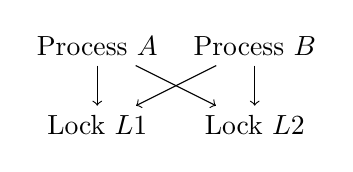
\begin{tikzpicture}[distance=5mm and 5mm]
    \special{dvisvgm:raw <g id="A">}
	\node (A) {Process $A$};
    \special{dvisvgm:raw </g>}
    \special{dvisvgm:raw <g id="B">}
	\node (B) [right of=A,xshift=10mm] {Process $B$};
    \special{dvisvgm:raw </g>}
	\node (L1) [below of=A] {Lock $L1$};
	\node (L2) [below of=B] {Lock $L2$};
    \special{dvisvgm:raw <g id="AL1">}
	\draw [->] (A) -- (L1);
    \special{dvisvgm:raw </g>}
    \special{dvisvgm:raw <g id="BL2">}
	\draw [->] (B) -- (L2);
    \special{dvisvgm:raw </g>}
    \special{dvisvgm:raw <g id="AL2">}
	\draw [->] (A) -- (L2);
    \special{dvisvgm:raw </g>}
    \special{dvisvgm:raw <g id="BL1">}
	\draw [->] (B) -- (L1);
    \special{dvisvgm:raw </g>}
\end{tikzpicture}% 
}


\end{document}